\documentclass[a4,12pt]{article}
\usepackage{colortbl}
\usepackage{pgfplots}
\usepackage[margin=2cm]{geometry}
\pgfplotsset{compat=newest}
\begin{document}
\begin{table}
\footnotesize
\sffamily
\begin{center}
\begin{tabular}{cccccc}
Mean-Accuracy & \shortstack{DefFCN \\ 0.8238} & \shortstack{No Modulation \\ 0.8237} & \shortstack{No DWSC \\ 0.8163} & \shortstack{Stripped \\ 0.8025} \\[1ex]
\shortstack{Stripped \\ 0.8025} & \bfseries \cellcolor[rgb]{0.3286,0.4397,0.8696}\shortstack{\rule{0em}{3ex} -0.0213 \\ 41 / 3 / 68 \\ 0.0033} & \bfseries \cellcolor[rgb]{0.3286,0.4397,0.8696}\shortstack{\rule{0em}{3ex} -0.0213 \\ 42 / 1 / 69 \\ 0.0056} & \cellcolor[rgb]{0.5217,0.6596,0.9877}\shortstack{\rule{0em}{3ex} -0.0138 \\ 60 / 1 / 51 \\ 0.4635} & \cellcolor[rgb]{0.8674,0.8644,0.8626}\shortstack{\rule{0em}{3ex} Mean-Difference \\ r$>$c / r=c / r$<$c \\ Wilcoxon p-value} \\[1ex]
\end{tabular}\\
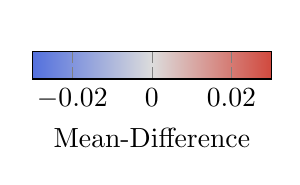
\begin{tikzpicture}[baseline=(current bounding box.center)]\begin{axis}[hide axis,scale only axis,width=0sp,height=0sp,colorbar horizontal,colorbar style={width=0.25\linewidth,colormap={cm}{rgb255(1)=(83,112,221) rgb255(2)=(220,220,220) rgb255(3)=(209,73,62)},colorbar horizontal,point meta min=-0.03,point meta max=0.03,colorbar/width=1.0em,scaled x ticks=false,xticklabel style={/pgf/number format/fixed,/pgf/number format/precision=3},xlabel={Mean-Difference},}] \addplot[draw=none] {0};\end{axis}\end{tikzpicture}\end{center}
\caption{[...] \textbf{If in bold, then p-value $<$ 0.05} [...]}
\end{table}
\end{document}
